Meg vive en Indianapolis y quiere visitar a su mamá en Lima,
como se muestran a continuación en la figura \ref{fig:proverb_pitagoras_07}
\begin{figure}[H]
    \begin{center}
        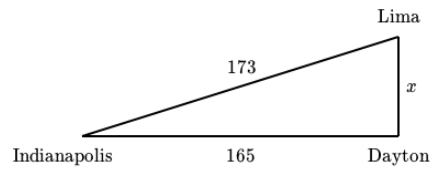
\includegraphics[width=0.5\textwidth]{../images/proverb_pitagoras_07}
    \end{center}
    \caption{}
    \label{fig:proverb_pitagoras_07}
\end{figure}
\textbf{¿Cuántos kilómetros más conduciría Meg si fuera a Lima pasando por Dayton?}\\


\begin{solutionbox}{12cm}
    Podemos usar el teorema de Pitágoras para obtener $x$.
    La ecuación del teorema de Pitágoras es:
    \[c^2=a^2+b^2\]
    donde $a$ y $b$ son las longitudes de los dos catetos del triángulo y $c$ es la longitud de la hipotenusa.
    En este caso, $a=x$, $b=165$ y $c=173$.
    \begin{align*}
        173^2        & =165^2+x^2     \\
        29,929       & = 27,225 + x^2 \\
        2,704        & =x^2           \\
        \sqrt{2,704} & =x             \\
        52           & = x
    \end{align*}
    Para calcular qué tan lejos es viajar a Lima pasando por Dayton, podemos sumar las distancias entre cada una de las ciudades.
    \[165+52=217\]
    Para calcular cuántos kilómetros más conduciría Meg si pasara por Dayton, podemos restar.
    \[217-173=44\]
    Meg conduciría 44 kilómetros adicionales si fuera a Lima pasando por Dayton.
\end{solutionbox}